\documentclass[11pt]{article}
\usepackage[a4paper, margin=2cm]{geometry}
\usepackage[utf8]{inputenc}
\usepackage{graphicx}
\usepackage{lastpage}
\usepackage{fancyhdr}
\usepackage{amssymb}

\pagestyle{fancy}
\fancyhf{}
\rfoot{Page \thepage \hspace{1pt} sur \pageref{LastPage}}

\begin{document}

\title{\textbf{Math - Les coniques : Synthèse}}
\author{Hovinne Noé}
\date{Avril 2020}
\maketitle
\tableofcontents

\newpage

\section{Introduction}

En géométrie euclidienne, une conique est une courbe plane algébrique, définie initialement comme l’intersection d'un cône de révolution (supposé prolongé à l’infini de part et d’autre du sommet) avec un plan. Lorsque le plan de coupe ne passe pas par le sommet du cône, la conique est dite non dégénérée et réalise l’une des courbes suivantes : ellipse, parabole ou hyperbole, caractérisées par un paramètre réel appelé excentricité ($e$).\footnote{\textit{Conique}, dans \textit{Wikipédia}, https://fr.wikipedia.org/wiki/Conique (Dernière consultation le 19/04/20).}

\begin{figure}[h]
    \textit{\caption{}}
    \centering
    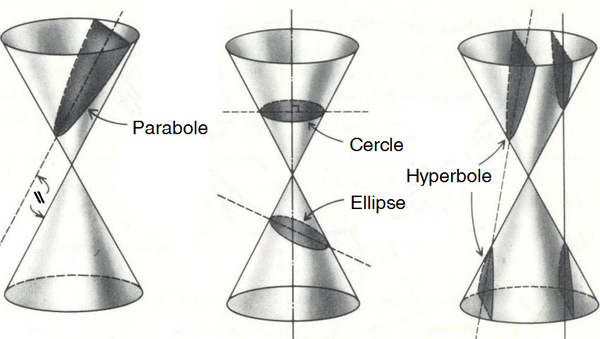
\includegraphics[width=6cm, height=3.39cm]{assets/coniques-synt-intro.png}
\end{figure}

\newpage

\section{Parabole}
\subsection{Définition de la parabole}
On appelle \textbf{parabole} le lieu des points du plan situés à égale distance d'une droite (la \textbf{directrice} de la parabole) et d'un point n'appartenant pas à cette droite (le \textbf{foyer} de la parabole).
\subsection{Équation de la parabole}
La parabole $\mathcal{P}$ de foyer $\displaystyle F \left( \frac{p}{2};0 \right)$ et de directrice $\displaystyle d \equiv x = -\frac{p}{2}$ a pour équation $y^2 = 2px$.

\newpage

\section{Ellipse}
\subsection{Définition de l'ellipse}
On appelle \textbf{ellipse} le lieu des points du plan situés à des distances de deux points fixes $F$ et $F'$ (les \textbf{foyers} de l'ellipse) dont la somme est constante.
\subsection{Équation de l'ellipse}
L'ellipse $\mathcal{E}$ de foyers $F$($c$ ; $0$) et $F'$($-c$ ; $0$) dont les points se trouvent à des distances de $F$ et $F'$ dont la somme vaut $2a$, avec $a>c$, a pour équation $\displaystyle \frac{x^2}{a^2} + \frac{y^2}{b^2} = 1$ avec $\displaystyle b^2=a^2-c^2$ $(b>0)$.

\newpage

\section{Hyperbole}
\subsection{Définition de l'hyperbole}
On appelle \textbf{hyperbole} le lieu des points du plan situés à des distances de deux points fixes $F$ et $F'$ (les \textbf{foyers} de l'hyperbole) dont la valeur absolue de la différence est constante.
\subsection{Équation de l'hyperbole}
L'hyperbole $\mathcal{H}$ de foyers $F$($c$ ; $0$) et $F'$($-c$ ; $0$) dont les points se trouvent à des distances de $F$ et $F'$ dont la valeur absolue de la différence vaut $2a$, avec $c>a$, a pour équation $\displaystyle \frac{x^2}{a^2} - \frac{y^2}{b^2} = 1$ avec $b^2=c^2-a^2$ $(b>0)$.



\end {document}